\subsection{Herzscher Dipol}
    "Elektrisches Pendel": Kondensator und Spule sind Energiespeicher.
    Wenn das magnetische Feld abgebaut wird, so wird das elektrische aufgebaut und umgekehrt.
    Idealisiert (ohne Reibung) "pendelt" dieses System unendlich lange
    \centering
    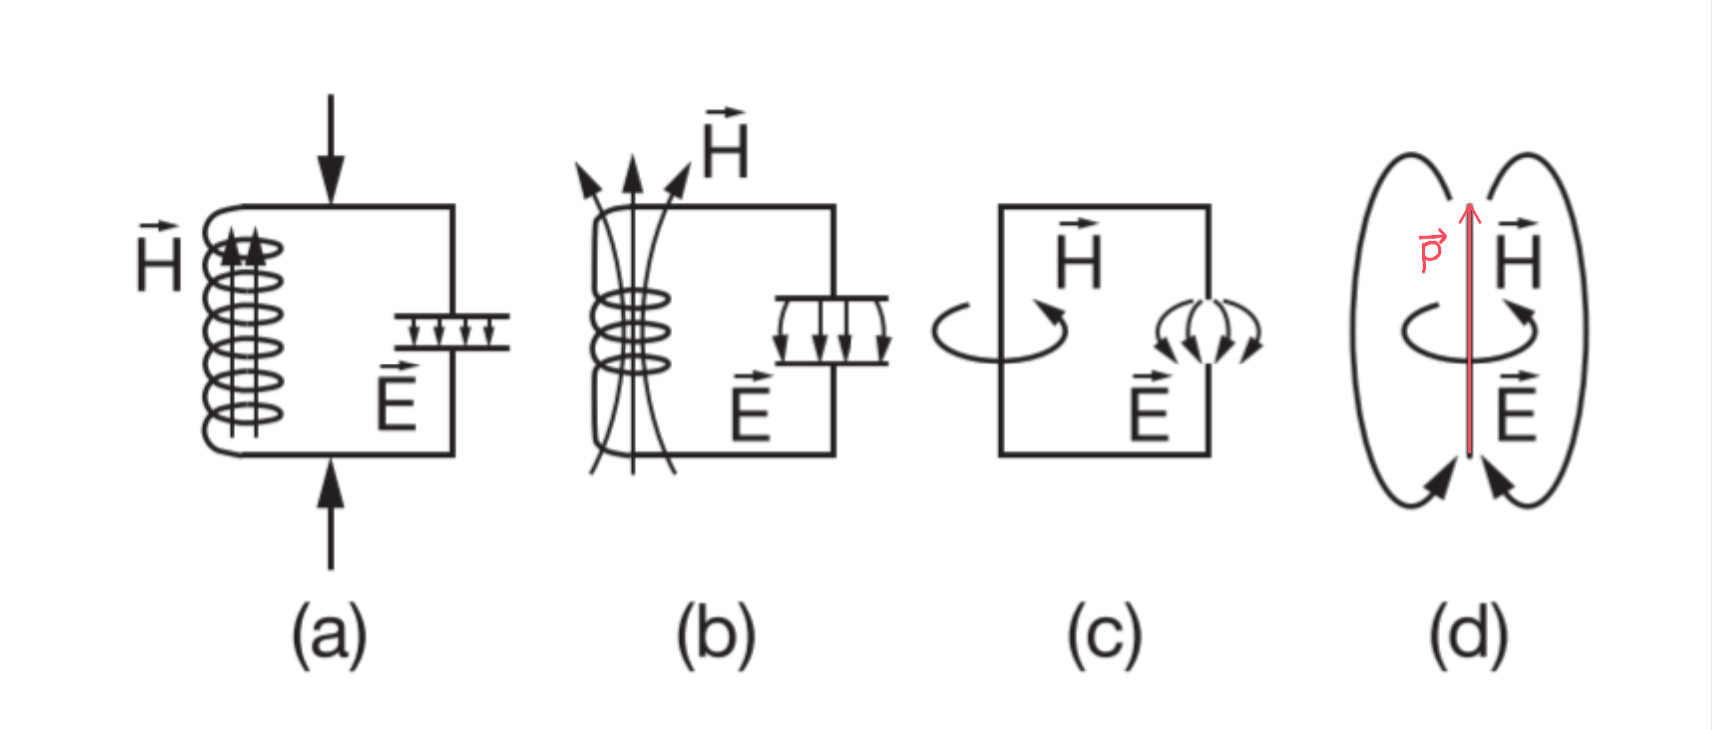
\includegraphics[height = 30mm]{src/images/herzscher_dipol.png}

    \begin{minipage}{0.49\linewidth}
        \begin{empheq}[box = \fbox]{align*}
            \vec{p} = q \vec{l} = \vec{p_0} cos(\omega t)\\
            \vec{E} = \vec{E_0} cos(\omega t - k r)\\
            \vec{H} = \vec{H_0} cos(\omega t - k r)
        \end{empheq}
    \end{minipage}
    \begin{minipage}{0.44\linewidth}
        \begin{scriptsize}
            \begin{empheq}{align*}
                \vec{p} &= \text{Dipolmoment (alternierende Richtung)}
            \end{empheq}
            Fernfeld: Entfernt man sich weit vom Sender (Herzschen Dipol), verschwindet der Phasenunterschied zwischen $\vec{E}$ und $\vec{B}$.
        \end{scriptsize}
    \end{minipage}
